\section{Theory \& Methods}
\subsection{Theory}

\subsubsection{Error Function}
The Error Function describes the probability that an observation lies within
a given interval, and can be seen in equation \ref{eq:1}.
\begin{equation} \label{eq:1}
    Erf(x)=\frac{2}{\sqrt{\pi}} \int_{-\infty}^x e^{-t^2} dt
\end{equation}

Where \(t=\frac{x}{\sqrt{\pi}}\). The error function is found by integrating
the normalised Gaussian distribution. The function is normalised by the
coefficient in front of the integral, so that \(erf(\infty) = 1\).
A visualisation of the error function from -3 $\leq$ x -3 $\leq$ 3 can be seen
in figure \ref{figure:error_function}

\begin{figure}[ht]
    \centering
    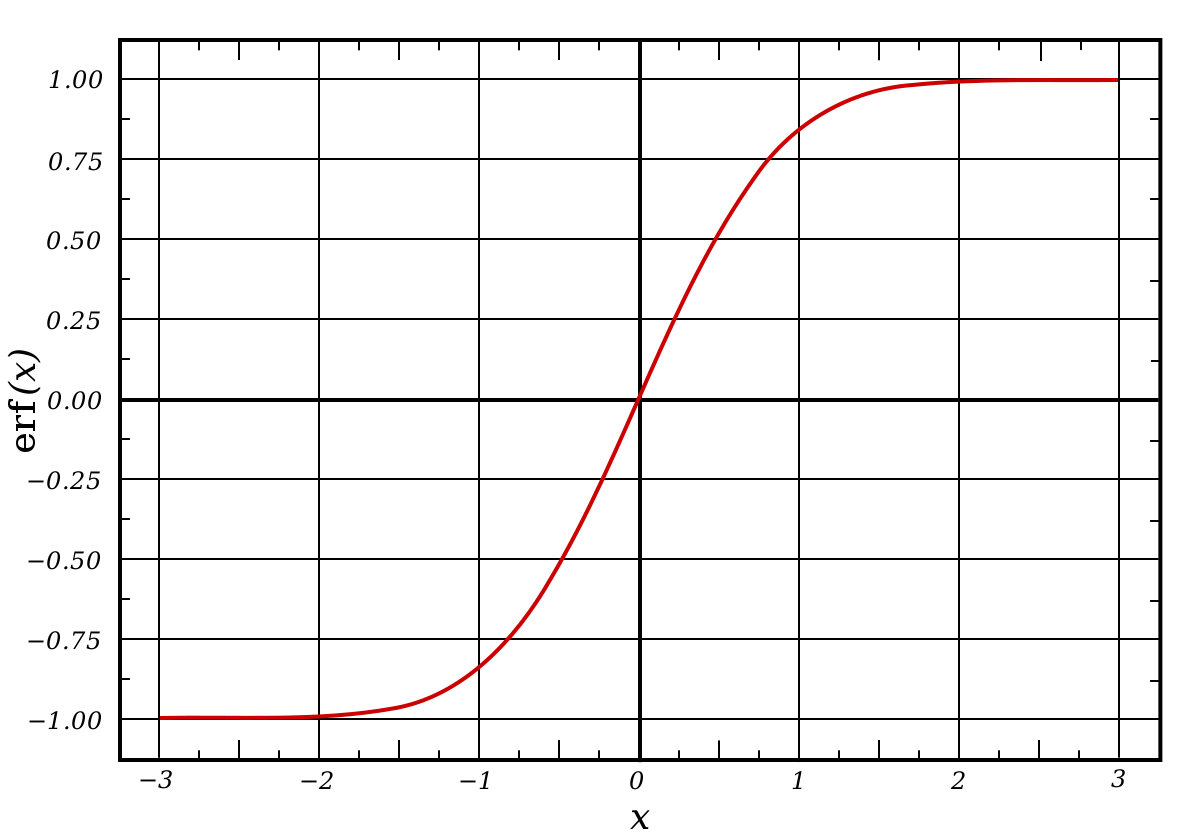
\includegraphics[scale=0.3]{images/error_function.png}
    \caption{Error function}
    \label{figure:error_function}
\end{figure}

\subsubsection{Overall Equipment Effectiveness}
The \textbf{O}verall \textbf{E}quipment \textbf{E}ffectiveness, OEE, is a
measurement of how effective a given production line is. It identifies what
percentage of the manufacturing time that is truly productive. The formula for
the OEE can be seen in equation \ref{eq:2}
\begin{equation} \label{eq:2}
    OEE = \frac{Good Count * Ideal Cycle Time}{Planned Produciton Time}
\end{equation}

Where \textit{GoodCount} is the amount of acceptable products produced and
\textit{IdeaCycleTime} is the theoretical minimum time to produce a single
product.

\subsection{Methods}
\subsubsection{SCRUM}
To keep track of the group work, the Scrum framework, with a few buts, is used.
Scrum consists of multiple artefacts and ceremonies, and in this project product
roadmap, Scrum meetings, product and sprint backlogs and burndown charts will
be used. Each sprint will have a duration of two weeks and the issues for the
sprint backlog will be chosen at the beginning of each sprint, at the Scrum
meeting. The Scrum meeting will take place each Friday and will be a mixture of
sprint planning, daily Scrum, and sprint review. To manage Scrum, ZenHub, a
management solution that can be integrated with GitHub, is used. On ZenHub the
group will create the roadmap, that acts as a schedule for the project and
board, which is where the issues will be handled. A burndown chart for each
sprint is automatically generated and kept up to date by ZenHub. The board will
consist of five columns, as seen below.

\begin{table}[H]
    \begin{tabularx}{\textwidth}{|>{\RaggedRight}X|>{\RaggedRight}X|>{\RaggedRight}X|>{\RaggedRight}X|>{\RaggedRight}X|>{\RaggedRight}X|>{\RaggedRight}X|}
        \hline                             
        \textbf{Product Backlog} & \textbf{Sprint Backlog} & \textbf{In Progress} & \textbf{Review/QA} & \textbf{Closed} \\
        \hline
        Issues & Issues for the given sprint & Issues that is currently being worked on & Issues that are pending (or in) review & Approved issues that have been merged    \\
        \hline
    \end{tabularx}
    \caption{Scrum Board} 
    \label{table:scrum}
\end{table} 

\subsubsection{MoSCoW}
MoSCoW is an important prioritising model used in software development, as it
describes which parts of the system that constitute the minimal viable product,
MVP. The use cases for the system to be developed are prioritised with the
costumer as this makes it clear which parts of the system to develop first.
These use cases are then presented in a table, to improve readability.\\

MoSCoW is an acronym standing for:\\

\begin{description}
    \item [Must have:] the use cases needed for the system to work and be
    accepted by the customer.

    \item [Should have:] what use cases the customer would like to have
    implemented, but they are not necessarily important for the system to work.

    \item [Could have:] use cases the customer would like to have implemented if
    there is enough time for it.

    \item [Won't have (this time):] use cases that is not to be prioritised in
    this iteration, but maybe in future releases.
\end{description}

\subsubsection{FURPS+}
FURPS+ is a model for classifying functional and non-functional requirements and
help giving a detailed description of the requirements. The acronym stands for:

\begin{description}
    \item [Functionality:] What the customer wants, including security measures.

    \item [Usability:] How effective is the product from the user's point of
    view? Is the product aesthetically acceptable? Is the documentation adequate?

    \item [Reliability:] What is the most acceptable system downtime? Are system
    errors predictable? Is it possible to demonstrate how accurate the results
    are? How is the system restored?

    \item [Performance:] How fast should the system be? What is the maximum
    response time? What is the throughput? How much memory does the system use?

    \item [Supportability:] Can the system be tested? Is it possible to
    configure the system, expand it, install it, and provide service on the
    system.
\end{description}

The + sign stands for supplementary needs the customer could have, and includes:

\begin{description}
    \item [Design constraints:] Do I/O devices or database management systems
    influence how the software should be built?

    \item [Implementation requirements:] Are there any standards the programmers
    must adhere to? is test-driven development necessary?

    \item [Interface requirements:] What downstream feeds need to be made? What
    other systems should the system work with?

    \item [Physical requirements:] What hardware should the system be
    implemented on?
\end{description}